\documentclass{report}
\usepackage[T1]{fontenc} % Fontes T1
\usepackage[utf8]{inputenc} % Input UTF8
\usepackage[backend=biber, style=ieee]{biblatex} % para usar bibliografia
\usepackage{csquotes}
\usepackage[portuguese]{babel} %Usar língua portuguesa
\usepackage{blindtext} % Gerar texto automaticamente
\usepackage[printonlyused]{acronym}
\usepackage{hyperref} % para autoref
\usepackage{graphicx}
\usepackage{indentfirst}
\bibliography{bibliografia.bib}

\begin{document}

%%
% Definições
%
\def\titulo{Misturador de Músicas}
\def\data{15/06/2018}
\def\autores{André Alves, Daniel Correia, Pedro Almeida, Pedro Valente}
\def\autorescontactos{(88811) andr.alves@ua.pt, (88753) dcorreia@ua.pt,\\
 (89205) pedro22@ua.pt, (88858)pedro.valente@ua.pt}
\def\departamento{Departamento de Electrónica, Telecomunicações e Informática}
\def\empresa{Universidade De Aveiro}
\def\logotipo{img/ua.pdf}
%

%%%%%% CAPA %%%%%%
%
\begin{titlepage}

\begin{center}
%
\vspace*{50mm}
%
{\Huge \titulo}\\ 
%
\vspace{10mm}
%
{\Large \empresa}\\
%
\vspace{10mm}
%
{\LARGE \autores}\\ 
%
\vspace{30mm}
%
\begin{figure}[h]
\center
\includegraphics{\logotipo}
\end{figure}
%
\vspace{30mm}
\end{center}
%

\end{titlepage}

%%  Página de Título %%
\title{%
{\Huge\textbf{\titulo}}\\
{\Large \departamento\\ \empresa}
}
%
\author{%
    \autores \\
    \autorescontactos
}
%
\date{\data}
%
\maketitle

\pagenumbering{arabic}


\tableofcontents
\listoffigures    % descomentar se necessário



\chapter{Introdução}
\label{chap.introducao}
O objetivo do projeto é a criação de um sistema que permita criar músicas através da
composição de pedaços de música. O projeto funciona a partir de um servidor do XCOA.
O sistema é composto por vários componentes, componentes estes que são:
\begin{itemize}
	\item Interface Web
	\item Aplicação Web
	\item Persistência
	\item Gerador de Músicas
\end{itemize}	

A Interface Web (\autoref{chap.interface}) é composta por quatro páginas HTML cada uma com um propósito prório a explicar mais à frente.

A página Início é uma pequena página inicial na qual o utilizador poderá ver aquilo que pode fazer neste site, assim como algumas informações sobre os autores e o local onde o projeto foi desenvolvido.
	
A Aplicação Web consiste num programa python que serve conteúdos estáticos, esta parte do trabalho serve como ponte para todos os outros componentes, para além disto tem também objetivos próprios a ser 
explicados mais à frente na \autoref{chap.aplicacao}.

A parte da Persistência consiste numa base de dados relacional e obtenção de dados da mesma, tudo isto será depois utilizado pela parte da Aplicação Web para registar as músicas criadas, os excertos que existem e os votos de cada um dos utilizadores, explicado em maior detalhe em \autoref{chap.persistencia}.

A parte do Gerador de Música deverá aceitar uma pauta na forma de um dicionário, gerando a música
especificada. Caso a geração tenha sucesso, a música deverá ser escrita no sistema de ficheiros. Deverá igualmente ser gerado um identificador com base no conteúdo, sendo este devolvido pelo módulo para persistência na base de dados. Este componente deverá suportar pelo menos 5 efeitos a aplicar no momento da geração
da música.

\chapter{Desenvolvimento}
\label{chap.desenvolvimento}
	
\section{Interface Web}
\label{chap.interface}
A Interface Web é composta por quatro páginas desenvolvidas através de e HyperText Markup Language (HTML), JavaScript (JS) e Cascading Style Sheets (CSS). 

A página \textit{Início} é uma página inicial, onde se encontra informação sobre o que poderá ser feito no site. Além de servir como ligação para as outras páginas, a página \textit{Início} tem também informação sobre os elementos que desenvolveram o projeto e o local onde o mesmo foi desenvolvido.

A segunda página do site é a página \textit{Músicas}. Nesta página estão todas as músicas produzidas/editadas por todos os utilizadores. É também nesta página que os utilizadores poderão votar músicas, apenas um voto por utilizador. O voto pode ser \textit{upvote} ou \textit{downvote} e pode ser alterado. 
No projeto esta página apenas vai ter uma música de exemplo mostrando que os votos funcionam. Isto deve-se a um problema no Gerador de Músicas.

Na terceira página estão todos os excertos de sons que podem ser utilizados para criar músicas no Gerador de Músicas, ordenados por ordem alfabética. Os excertos podem também ser transferidos individualmente.

A quarta página do site diz respeito ao \textit{Misturador}. É nesta página que o utilizador pode misturar excertos criando uma música. Essa música depois de criada aparece na página das \textit{Músicas}, já em cima descrita. 
Ao misturar as músicas, o utilizador controla o número de batimentos por minuto da música assim como a adição de efeitos ao som e o volume.

No projeto, ao selecionar os excertos, o números de batimentos, o volume e os efeitos e ao clicar no botão \textit{Mistura-te!} é criado um ficheiro JSON (o ficheiro JSON é criado no ficheiro \textit{\texttt{get\_sheet.js}} através da função \textit{\texttt{generate\_json()}}) com todas as especificações selecionadas mas não é possível criar de facto a música. 


\section{Aplicação Web}
\label{chap.aplicacao}
A aplicação Web é o programa em python que serve como ponte entre todas as partes do projeto.
Tem as funções list, get, sheet e vote:

\subsection{list}
A função \textit{list} está dividida nas \textit{samples} e nas \textit{songs}.
\paragraph{Samples}
Este módulo quando usado vai devolver o JSON de todas as samples com o 
\textit{name, date, id, length} das samples guardado na base de dados na tabela de Samples.
\paragraph{Songs}
À semelhança do módulo das Samples, este irá devolver o JSON de todas 
as músicas criadas com o \textit{name, date, id, length, uses, votes, author}
 que também se encontra guardado na base de dados.
 \paragraph{Aceder}
	Para aceder deve-se escrever \textit{/list?type=songs} para o JSON de músicas e \textit{/list?type=samples}
 para os das samples
 \subsection{get}
 Esta função devolve todos os atributos de uma sample ou song através do seu id.
 \paragraph{} Não se encontra funcional.
 \paragraph{Aceder} 
 Para aceder deve-se escrever \textit{/get?id=id} em que o id é uma string de 16 caracteres de 0 a 9 e de A a F.

 \subsection{sheet}
 Esta função deveria fazer a mistura das samples para criar músicas.
 \paragraph{} Não se encontra funcional.

 \subsection{vote}
Função onde recebendo o id da música e os pontos(-1 ou 1) adiciona 
um voto negativo ou positivo na música.
A função averigua se o utilizador já votou ou não. Caso já tenha votado
dá para tirar o voto clicando no botão contrário ao usado para votar e
poderá votar denovo.
A função adiciona os votos diretamente na base de dados.



\section{Persistência}
\label{chap.persistencia}
Este projeto contém uma base de dados que recorre à utilização de três tabelas, todas as tabelas são alteradas consoante as funções de Python existentes no resto do projeto.
Tabelas estas que vão de seguida enviar os dados para as páginas HTML através de JavaScript.
A tabela das samples serve para guardar todos os excertos que colocámos disponíveis.
Esta tabela tem como componentes:
	\begin{itemize}
		\item Name   -> do tipo TEXT
		\item Date   -> do tipo TEXT
		\item ID     -> do tipo TEXT
		\item Length -> do tipo INTEGER
		\item Uses   -> do tipo INTEGER
	\end{itemize}


A tabela das músicas serve para guardar todas as músicas criadas pelos utilizadores Misturador, esta tabela deverá conter apenas uma amostra exemplar, isto porque o nosso misturador não funcionava pelo que esta tabela não irá receber dados.
Esta tabela terá também uma contagem de votos assim como o autor de cada uma das músicas.
Esta tabela tem como componentes:
	\begin{itemize}
		\item Name -> do tipo TEXT
		\item Date -> do tipo TEXT
		\item ID -> do tipo TEXT
		\item Length -> do tipo INTEGER
		\item Uses -> do tipo INTEGER
		\item Votes -> do tipo INTEGER
		\item Author -> do tipo TEXT
	\end{itemize}

A tabela dos votos irá ter a função de guardar os votos que são inseridos em cada uma das músicas, cada utilizador apenas pode ter um voto numa música(pode votar 1, -1 ou deixar 0 se se quiser manter imparcial).
É permitido ao utilizador alterar o seu voto.
Esta tabela tem como componentes:
	\begin{itemize}
		\item Email -> TEXT
		\item sID -> TEXT
		\item Points -> INTEGER
	\end{itemize}

\newpage

\section{Gerador de Músicas}
\label{chap.gerador}
Como já foi referido \autoref{chap.interface} o Misturador de Músicas não está totalmente funcional. A seleção dos excertos, dos efeitos, do volume e dos batimentos por minutos está operacional e é criado um ficheiro JSON com toda essa informação. O ficheiro JSON é criado no ficheiro \textit{\texttt{get\_sheet.js}} através da função \textit{\texttt{generate\_json()}}). A informação que entra no ficheiro JSON é conseguida através das funções \textit{\texttt{get\_samples()}} (excertos), \textit{\texttt{get\_effects()}} (efeitos) e \textit{\texttt{get\_vol()}} (volume).

O aspeto do misturador é o seguinte:

	\begin{figure} [h]
		\centering
		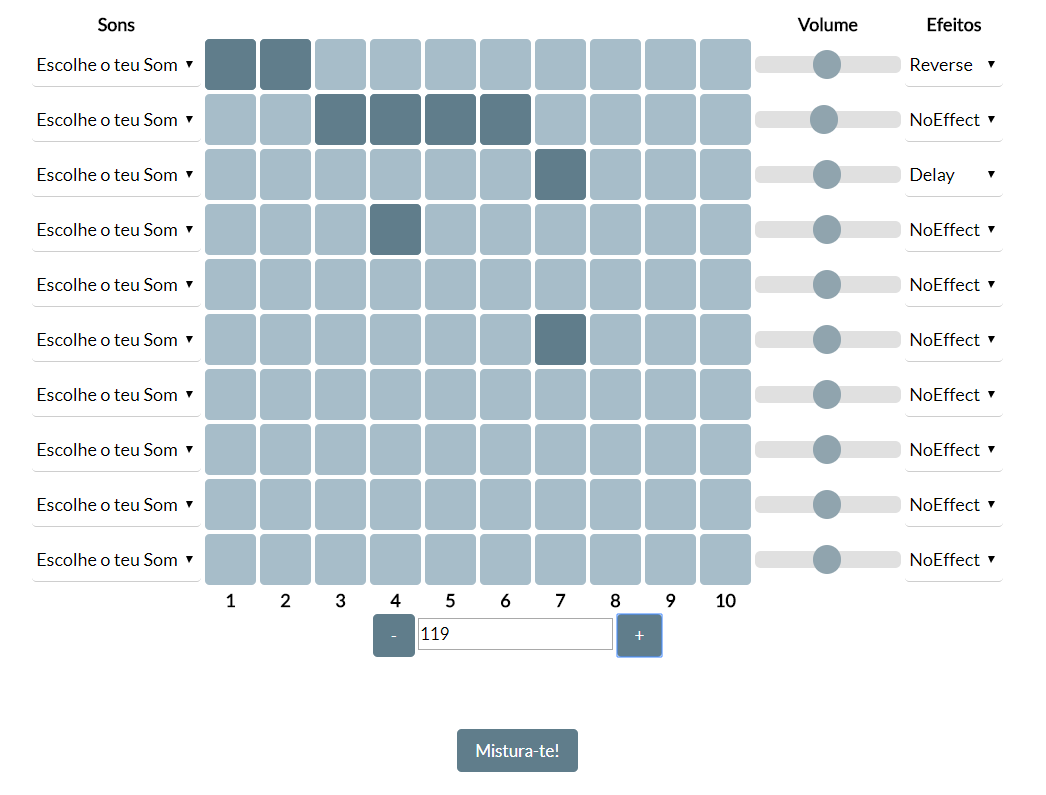
\includegraphics[scale=0.5]{img/misturador.PNG}
		\caption{Misturador de músicas}
	\end{figure}

O que falta para o Misturador de Músicas estar a funcionar é passar a informação do ficheiro JSON para python e usar a função \textit{mix()} (esta já criada no ficheiro \textit{mixer.py}).

\chapter{Resultados}
\label{resultados}

\section{Demonstração do funcionamento dos Votos}
\begin{figure} [h]
	\centering
	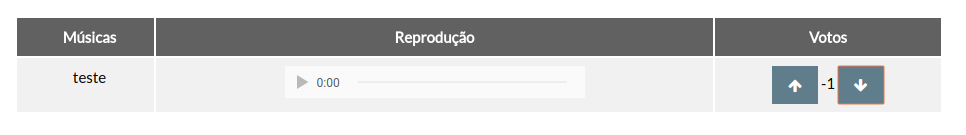
\includegraphics [scale = 0.4] {img/votos-1}
	\caption{Resultado dos votos para: -1}
\end{figure}

\begin{figure} [h]
	\centering
	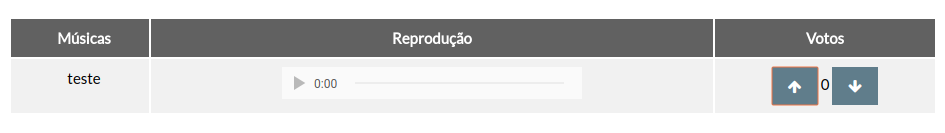
\includegraphics [scale = 0.4] {img/votos0}
	\caption{Resultado dos votos para: 0}
\end{figure}

\begin{figure} [h]
	\centering
	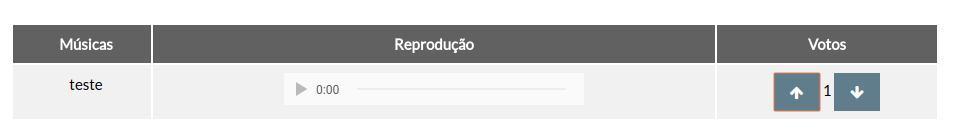
\includegraphics [scale = 0.4] {img/votos1}
	\caption{Resultado dos votos para: 1}
\end{figure}

\section{Demonstração do funcionamento da página Excertos}
\begin{figure} [h]
	\centering
	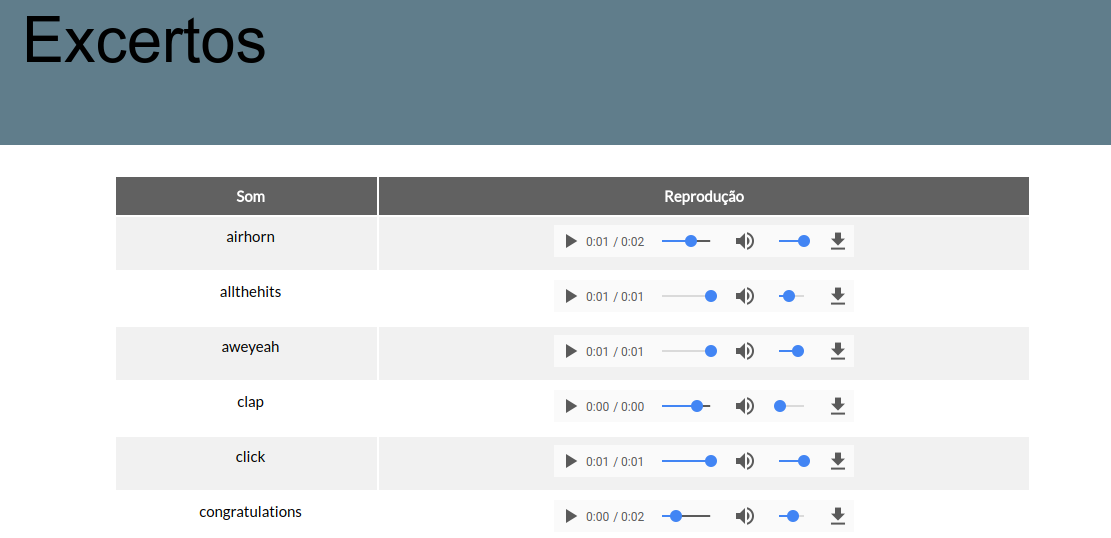
\includegraphics [scale = 0.3] {img/excertos}
	\caption{Funcionamento de todos os componentes da página excertos}
\end{figure}

\newpage
\section{Demonstração do funcionamento da Base de Dados}
\begin{figure} [h]
	\centering
	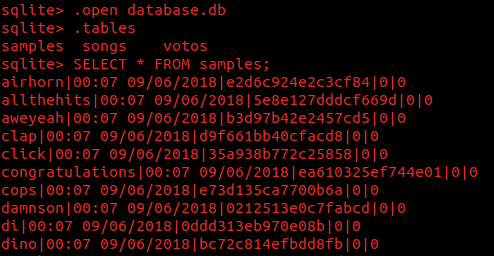
\includegraphics [scale = 0.4] {img/samples}
	\caption{Funcionamento da tabela samples}
\end{figure}

\begin{figure} [h]
	\centering
	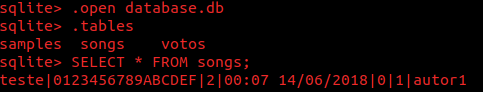
\includegraphics [scale = 0.5] {img/songs}
	\caption{Funcionamento da tabela songs}
\end{figure}

\begin{figure} [h]
	\centering
	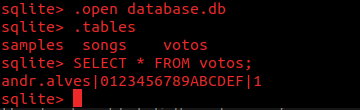
\includegraphics [scale = 0.5] {img/votos}
	\caption{Funcionamento da tabela votos}
\end{figure}

	 
\chapter{Conclusões Finais}
\label{chap.conclusao}
	Com este projeto de gerador de músicas foi possível consolidar os conhecimentos adquiridos em aulas pois foi necessário tudo o que foi realizado ao longo semestre. 
	
	Infelizmente, o projeto não está completamente funcional. Ainda assim, com o que foi feito, mudou a forma como os elementos do grupo veem as aplicações como esta de gerador de músicas, todo o trabalho que está por detrás do que é apresentado ao utilizador.  
	
	No futuro o que o grupo pode melhorar é a gestão de tempo pois foi isso que impossibilitou a conclusão do projeto na íntegra.


\chapter{Contribuições dos autores}
\label{contribuições}

\noindent
André Alves - 25\% \\
Daniel Correia - 25\% \\
Pedro Almeida - 25\% \\
Pedro Valente - 25\% 


\end{document}